% !TEX encoding = UTF-8 Unicode
% ÄÖÜ ß äöü

\section{Architecture}

The general design of Ny$\bar{a}$ya follows the Model-View-Controller pattern,
which is originated in Smalltalk \cite[p.4]{GAMMAETAL} (like the Objective-C syntax)
and separates the representation of data from the user interaction.
Cocoa \seeref{sec:Cocoa} encourages the use of MVC by providing a rich set of useful views and controllers.
Those cover many use cases of data presentation and user interaction. 

\section{Model}

Ny$\bar{a}$ya must hold different representations of Boolean functions – propositional formulas, abstract syntax trees and binary decision diagrams. 

\subsection{Formulas}
Propositional formulas and Boolean expressions are subsets of the set of all Unicode strings. 
Therefore they are easily represented by the Cocoa Foundation's \seeref{secitem:CocoaFoundation} 
standard string class. 

Due to the unambiguous relationship between propositional formulas and Boolean expressions Ny$\bar{a}$ya allows the use of a mixed syntax and additional symbols for the user's convenience. 


\subsection{Abstract Syntax Trees}

Cocoa Touch Foundation does not provide a class to represent trees, 
but with an class implementing the composite pattern \cite[p.163ff]{GAMMAETAL}
arbitrary graphs and therefore trees can be represented easily.

\begin{figure}[htbp]
\begin{center}
\UML{NyayaNode.png}
\caption{node class to represent an abstract syntax tree}
\label{fig:NyayaNodeCluster}
\end{center}
\end{figure}

The node class is implemented as an class cluster, 
which is an Cocoa design pattern \cite[p.282ff]{Buck:2009:CDP:1803585}
– an application of the the abstract factory design pattern \cite[p.87ff]{GAMMAETAL}.
The abstract and public class \verb+NyayaNode+ 
provides a set of static and public methods (see \figref{fig:NyayaNodeCreation}),
that returns instances of non public sub-classes (see \figref{fig:NyayaNodeCluster})
of \verb+NyayaNode+.

\begin{figure}[htbp]
\begin{center}
\UML{NyayaNodeCluster.png}
\caption{public root class and non public subclasses}
\label{fig:NyayaNodeCluster}
\end{center}
\end{figure}



Actual the creational methods are implemented as class category, 
which is a language feature of Objective-C \cite[p.225ff]{Kochan:2009:PO:1538451}
– an application of the decorator design pattern \cite[p.175ff]{GAMMAETAL} –
for extending the functionality beyond representing a tree. 

\begin{itemize}
\item Attributes
\item Creation  (see \figref{fig:NyayaNodeCreation})

\begin{figure}[htbp]
\begin{center}
\UML{NyayaNodeCreation.png}
\caption{Creation of nodes}
\label{fig:NyayaNodeCreation}
\end{center}
\end{figure}

\item Derivations
\item Description
\item Display  % (see \figref{fig:NyayaNodeDisplay)
\item Random
\item Reductions
\item Resolution
\item Transformations
\item Type
\item Valuation (see \figref{fig:NyayaNodeValuation})

\begin{figure}[htbp]
\begin{center}
\UML{NyayaNodeValuation.png}
\caption{Valuation of trees}
\label{fig:NyayaNodeValuation}
\end{center}
\end{figure}

\end{itemize}





\begin{figure}[htbp]
\begin{center}
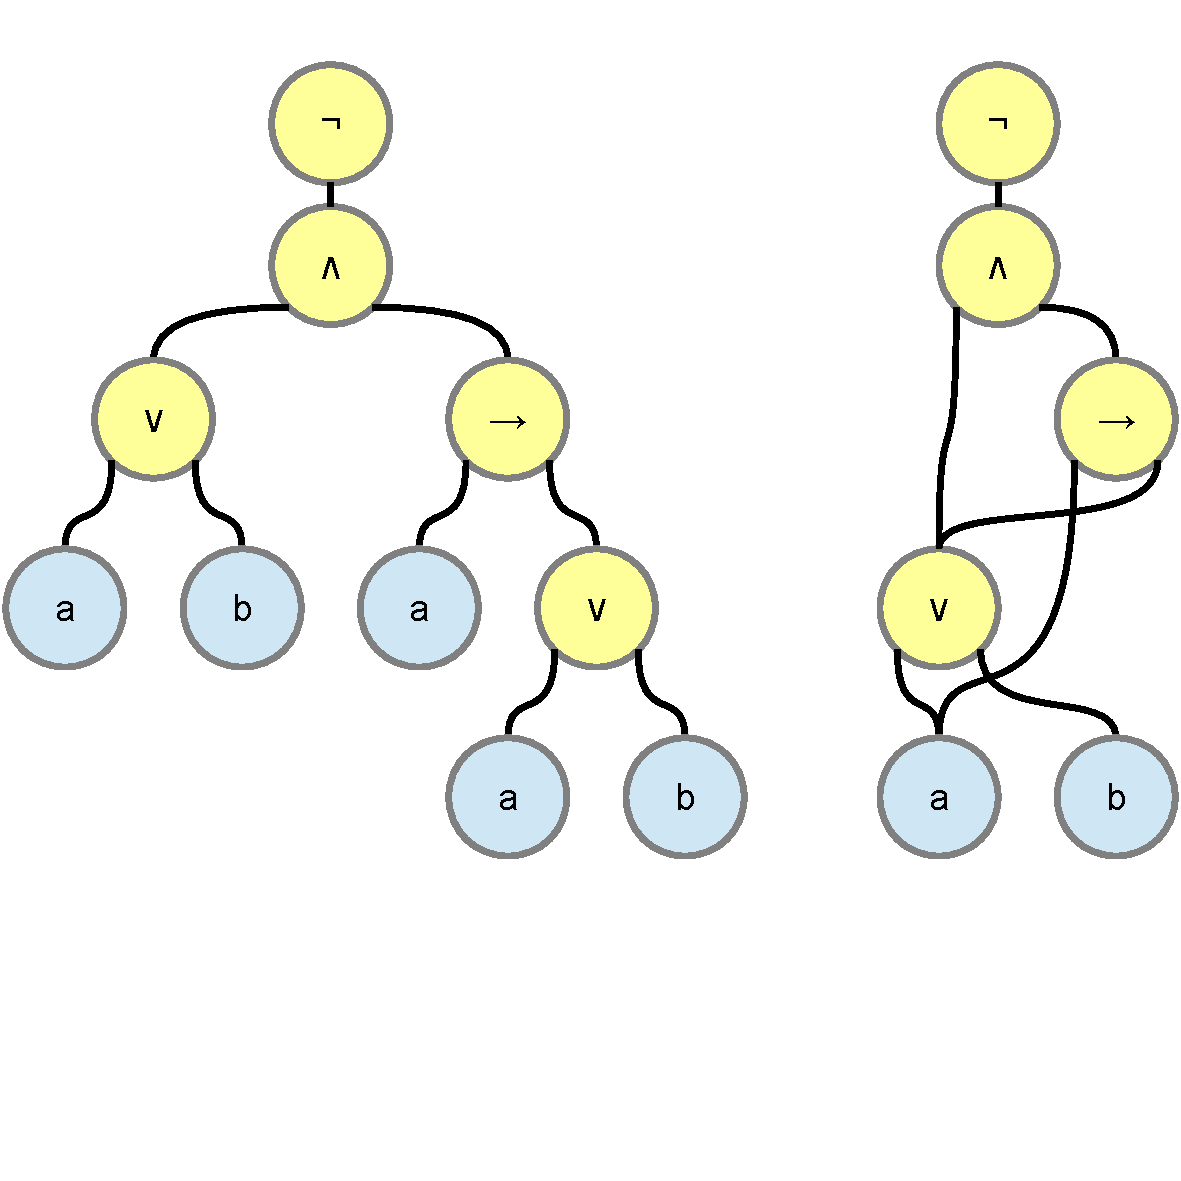
\includegraphics[scale=0.5]{diagrams/AcyclicSyntaxGraph.pdf}
\caption{Abstract syntax tree and internal representation}
\label{fig:NyayaNodeDisplay}
\end{center}
\end{figure}

\subsection{Binary Decision Diagrams}

\subsection{Parser}


\cite{Louden:1997:CCP:523017}

\begin{table}[htdp]
\begin{center}
$\top | \bot 
| \neg | !
| \wedge | \& | .
| \vee | {\setminus}| | {\setminus}+ 
| \veebar | \oplus | \textasciicircum
| = | <> | \leftrightarrow 
| > | \rightarrow | \models
| ( | ) | , | ; 
| {\setminus}w+$ 
\caption{Regular expression for the lexxer of Ny$\bar{a}$ya}
\label{tab:REGEX}
\end{center}
\end{table}


The set of valid sub-strings (symbols and identifiers) is defined by a regular expression (see \tabref{tab:REGEX}). 
The input string is split into tokens by the standard regular expression class of Cocoa Foundation.

\begin{table}[htdp]
\begin{center}
\begin{lstlisting}[mathescape]
formula        ::= entailment
entailment     ::= sequence [ $\models$ entailment]
sequence       ::= bicondition { ; bicondition } 
bicondition    ::= implication [ $\leftrightarrow$ bicondition ]
implication    ::= xdisjunction [ $ \rightarrow$ implication ]
xdisjunction   ::= disjunction { $\veebar$ disjunction }
disjunction    ::= conjunction { $\vee$ conjunction }
conjunction    ::= negation { $\wedge$ negation }
negation       ::= $\neg$ negation | ( formula ) | identifier
\end{lstlisting}
\caption{EBNF grammer for the parser of Ny$\bar{a}$ya}
\label{tab:EBNF}
\end{center}
\end{table}


\section{Views}

\begin{figure}[htbp]
\begin{center}
\UML{TreeView.png}
\caption{Tree viewr}
\label{fig:TreeView}
\end{center}
\end{figure}

\begin{figure}[htbp]
\begin{center}
\UML{NyayaNodeDisplay.png}
\caption{Node display interface}
\label{fig:NyayaNodeDisplay}
\end{center}
\end{figure}

\section{Controllers}








\section{Unit-Tests}

\section{Content}



